%!TEX root=../thesis.tex

\chapter[Proposal]{Proposal} \label{chap:proposal-phd}
\footnote{The structure follows \citeauthor{Schmitter2002}'s suggestions for a good PhD proposal \citeyearpar{Schmitter2002}.
    }

\begin{quote}
    \emph{``The spirit of a people, its cultural level, its social structure, the deeds its polity may prepare --- all this and more is written in its fiscal history, stripped of all phrases.
    He who knows how to listen to its message here discerns the thunder of world history more clearly than anywhere else.''}\\
    --- Joseph \citet[6]{Schumpeter}
    %add better source
\end{quote}

\begin{quote}
    \emph{``The unforced force of the better argument'':}\\
	%\cite[305]{Habermas1996}
    \emph{``The speaker must choose a comprehensible expression so that speaker and hearer can understand one another.''}\\
    %\cite[2f]{Habermas1976}
    \emph{``[A]nyone acting communicatively must, in performing any speech act, raise universal validity claims and suppose that they can be vindicated.''}\\
	%\cite[2]{Habermas1979}
    --- Jürgen Habermas (\citeyear[305]{Habermas1996}, \citeyear[2f]{Habermas1976}, \citeyear[2]{Habermas1979}, respectively)
\end{quote}

%write one short sentence, follow with several paragraphs to explain (schmitter)
%1. The idea: what do you want to study?
%2. The reason: why do you want to study it? 

\section{Introduction}
If world history is still written in tax, as \citeauthor{Schumpeter} believed, the people of our democracies, too, must read and speak these codes, to live up to the emancipatory promise of modernity.
If communicative action can heal the disagreement and confusion wrought as modernity differentiated System and Lifeworld, as \citeauthor{Habermas-1984-aa} hopes, in our discourse on tax, too, universally acceptable validity claims instead of money and power must rule to uphold our faith in liberal democracy.

I here propose to probe into one intersection of legitimate inputs and outputs of the social contract: the discourse \emph{on}, and economics \emph{of} tax.

I ask, how --- if at all --- do people under current democratic arrangements think differently about tax, from how they \emph{would} think about it, if they lived under conditions of ideal speech.
I test, how --- if at all --- do people change their thinking about tax, if they participate in a democratic process that is \emph{closer} to the Habermasian ideal?

\subsection{Taxation and Welfare}
Why does taxation matter for human welfare?

As \citeauthor{Schumpeter} knew, ``in the modern world, taxation \emph{is} the social contract'' \citep[1, emphasis in original]{Martin2009a}, even though social scientists have since paid little attention to it \citep[K191]{Tilly2009}.
This is especially true of current \gls{OECD}-style welfare regimes, in which markets and states must co-exist. %find general reference
In such a mixed economy, government must be able to draft some privately-owned resources to serve its --- ideally democratic --- \emph{command}, without unduly altering the prices of --- ideally competitive --- \emph{exchanges} \citep[165f]{Ardant1975}.
Much of modern social integration occurs in the balance of these two contrasting logics to produce and allocate resources, ``enmesh[ing] us in the web of generalized reciprocity that constitutes modern society'' \citep[3]{Martin2009a}.
State plans make the conditions \emph{for}, and set limits \emph{to} \emph{individual} action, as when government builds roads or collects sewage fees.
Conversely, market exchanges produce much of the ``fungible resources'' used for \emph{collective} choice, as when pays road builders or procures sewage pipes \cite[4]{Martin2009a}.

Of all conceivable institutions to govern the interface of states and markets, taxation --- not price controls, not expropriation, not debt, not printing money, not tariffs --- is the most equitable, efficient and sustainable \citep{MusgThet1959,Stiglitz2011}. %add ref
Welfare states, with their penchant for market interventions for equity, efficiency \emph{and} sustainability, especially, rely on good taxes. %find quote about outcomes.

Instead, taxation everywhere in the \gls{OECD} is in crisis.
As alternative sources of economic relief --- monetary expansion and sovereign debt --- are maxed out, structural misalignments persist, and previously forestalling (asset) bubbles have burst into their days of reckoning, public revenues appear to be strictly limited by the longtime coming contradictions of current tax regimes. %add source
The popular mixture of (progressive) income, (proportional) consumption and (regressive) payroll taxes appears to offer only harshly unattractive tradeoffs between equity and efficiency, as bases have shrunk and schedules flattened \citep{Ganghof2006}.
If governments cannot raise the resources necessary to meet democratic demands without incurring prohibitive costs, the social contract is fraying \citep{Crouch2004}.%so so shource
Whichever way governments now turn, absent better tax, they will violate the post-war capitalist compact of stable, widely shared growth \citep{Pierson2002,StreeckMertens2010}. %so-so source

\subsection{Deliberation and Democracy}
Why does deliberating taxation matter for democracy?

A dysfunctional mixed economy without good taxes may produce illegitimate outputs, and, in so far as it disturbs the state-market balance of the mixed economy, violate congruency. %find source
Yet, even if experts could agree on a tax --- such as a promising, post-paid, cash-flow based \gls{PCT} --- the tradeoffs involved in choosing or calibrating a tax regime are irreducibly political.
For example, experts cannot \emph{positively} inquire whether economic ``growth''
\footnote{
	More precisely, the reaping of greater non-zero-sumness from social integration.%add source
} 
is in itself \emph{virtuous}, which inter-subjective aggregation would be \emph{utility-maximizing}, what \emph{deontological} rights owners have or which human \emph{relationships} should be governed by prices or command at all --- even if they could agree on any of those alternative ethics. %add hrefs
These metaphysical conundrums are reflected in very concrete, technocratic issues in taxation, including \glspl{DWL}, diminishing returns, capital income, or joint spousal taxation, respectively. %add hrefs
Likewise, experts cannot justify the axioms on which their (economic) analyses rest: whether, and under which institutional circumstances we are homines oeconomici, cannot be exhaustively answered from observation, because nature offers no intelligible moral messages on what kind of man we \emph{should} be. %add hrefs, source
This ontological stance matters for tax, too: for an expert to model a general equilibrium is to invoke, as well as to make, a homo economicus.

Of all conceivable institutions to resolve these disagreements, deliberative --- not aggregative, not pluralist, not participatory --- democracy offers the greatest normative appeal, because
these disagreements raise, in \citeauthor{Habermas-1984-aa}'s words, competing \emph{validity claims}, in need of argumentative redemption, as in: is ``growth'' \emph{comprehensible}, who \emph{truly} bears a \gls{CIT}, is homo economicus \emph{right}, and are social insurance employer co-payments \emph{truthful}?
Liberal democracy, borne out of the hope that material inequality and political autonomy \emph{can} be reconciled, %need quote 
especially, rests on deliberation, because if anywhere, it is in taxation that money and power may have replaced language to govern meaning and action.
In fact, if you wanted to hide some process of (re)producing inequality anywhere, you could hardly find a better place than the intricacies of (income) taxation.

Instead of communicative action \citep{Habermas-1984-aa}, what emerges today from citizens, their legislatures and public spheres, may be more ``analytic muddle of tax'' \citep[862]{McCaffery2005}.
The beliefs held and issues considered in the public \citep[for example,][]{Caplan2007}, appear to bear little resemblance to the abstractions suggested by economists \cite[for example,][]{Harberger1974}.
People seem to ignore fundamental choices in tax \citep[for example,][]{McCafferyHines2010}, and may fall for inconsequential alternatives \citep[for example,][]{SausgruberTyran2011}, possibly even err systematically against their own material interest --- if they are on the lower economic rungs \citep[for a German example,][]{Kemmerling2009}.

\subsection{Raw and Enlightened Thinking}

I here propose to investigate a supposed difference in current, and (more) ideal speech thinking about tax by subjecting a group of diverse citizens to a deliberative forum on the topic, which, in one canonic definition \cite[K1799]{Fishkin2009}, is marked by 
\begin{enumerate}
	\item reasonably accurate and complete \emph{information},
	\item substantive \emph{balance} of possibly competing arguments and perspectives presented,
	\item \emph{diversity} of participants and their positions taken,
	\item a sincere weighting of arguments by participants, or \emph{conscientiousness}
	\item equal consideration of all arguments, regardless of which participant offered them.
\end{enumerate}

%or, in Habermas terms, summarized by \cite[25f.]{Steenbergen2003}, a particularly succinct formulation of Habermas' endeavour
	%open participation Habermas 1992: 370-372)
	%justification Habermas 1992: 370
	%consider the common good, empathy, other-directedness, solidarity (Rawls 1971)
	% respect (gutmann and thompson 1996)
	% constructive politics, ``ideal deliberation aims to arrive at a rationally motivated consensus'' )Cohen 1989: 23)
	%authenticity (Habermas 1981: 149)
	
	%\cite{Steenbergen2003} but then, they sort of move from Habermas to whether there are none, incompletely linked, one or two justifications. \cite[28]{Steenbergen2003}

Such a difference $\Delta$ between ``raw'' and ``enlightened'' thinking, %cite mccaffery 
beliefs \citep{Caplan2007} and preferences \citep{Fishkin2009} is worth knowing for several reasons:
\footnote{
	\cite{PrzeworskiSalomon1995} suggest to explicate what readers are going to learn as a result of the proposed project, and why that would be worth knowing.
}
\begin{enumerate}
	\item 
		There may be \emph{agreeable}, doable but hypothetical taxes, which may (Pareto)-improve over current taxes \citep{Harberger1974} or may be fairer \citep{Rawls-1971-aa} and more sustainable \citep{Solow1956}, including a \glsfirst{PCT} \citep{Mill1848,McCaffery2002,Frank2005a,Seidman1997}, a \glsfirst{LVT} \citep{George1879,Buiter1988} and a \glsfirst{NIT} \citep{Friedman1962}.
		By comparison, existing taxes
		\footnote{
			In the \gls{OECD}-world, those are varying combinations of pre-paid, proportional consumption taxes such as \gls{VAT} and income taxes, often with different schedules for labor, capital and corporate incomes. Wealth taxes, often only on some asset classes, exist in some jurisdictions, but --- with the exception of local US property taxes --- are not a large revenue source.}
		appear unnecessarily wasteful, inequitable and unsustainable.
		These suboptimal tax regimes may present democratic sovereigns with needlessly harsh tradeoffs between efficiency, equity, sustainability and other competing ends.
		The means of an intact mixed economy \citep{MusgThet1959,Stiglitz2011} may consequently erode or even force retrenched welfare states into ``permanent austerity'' \citep{Pierson2002,StreeckMertens2010} as it becomes harder for them to reconcile planned allocation and market exchange through taxation.
		
		Public confusion about taxation may be a contributing factor, or even a sufficient --- but not a necessary --- condition for the non-existence of these supposedly superior taxes. 
	\item
		Progressivity in tax, especially, may hinge upon an enlightened, ``new understanding of tax'' \citep{McCaffery2005}, as the historic mainstay of redistribution --- the \gls{PIT} --- withers away in the face of its inherent contradictions \citep{McCafferyHines2010}.
		People may understand tax \emph{systematically} different from how they would under (more) ideal speech, which may cause them to choose less effectively progressive taxes than they otherwise might, or otherwise inadvertently act even against their material self-interest.
		Additionally, the difference between raw and enlightened thinking about tax may, in itself, depend on the socio-economic status of citizens.
		Taken together, such socially structured and structuring differences in understanding tax may contribute to further, or perpetuate existing social inequality, even under nominal political equality.
	\item
		The aggregative and representative institutions of liberal-pluralist democracy may be partly outmatched by the vexing complexity \citep{Merton-1968-aa} and tightly concentrated interest \citep{Olson-1971-aa} of late market economies, such as in taxation, violating both their input and output legitimacy \citep{Scharpf1997} as well as basic democratic prescriptions for ``enlightened understanding'' \citep{Dahl-1989-aa}.
		Empirical political sociology bears out such popular dissatisfaction, not with democracy it self, but with incumbents, enamored by special interest, and inattentive to the public good \citep{NyeJr.1997,Norris2011,PutnamPharr-2000-aa}.
		If such a ``post-democratic'' constellation \citep{Crouch2004} were to plague the polity in its thinking about tax, it may well affect other policy areas too.
\end{enumerate}

\section{State of the Field}
This positive aspect of this thesis sits at the intersection of two fields of empirical research: 
\begin{enumerate}
	\item Practical experiments with different deliberative fora on varying policy areas,
%	\item Political psychology on limited and socially structured cognitive competences and
	\item Experimental and survey research about popular understandings of tax.
\end{enumerate}

In the following, I briefly report key findings from these two fields and identify avenues for further research.

\subsection{Empirical Deliberation}

\subsubsection{Deliberative Experiments}
Deliberative fora have been tried on a number of policy areas and places, including renewable energy in Texas (USA) \citep{LehrGuild-2003-aa}, participatory budgeting in Porto Allegre \citep{CoelhoPozzono-2005-aa} (Brasil), nanotechnology \citep{Powell2008}, electoral reform in British Columbia (Canada), policing and education in Chicago (Illinois) \citep{WarrenPearse-2008-aa}, and city planning in Philadelphia (Pennsylvannia) \citep{Sokoloff2005}. 
They also vary in their institutional design \citep[reviewed in][]{Fung-2003-ac}.
These include several small-n, multi-day designs, such as Citizen Juries \citep{SmithWales-2000-aa} or Planning Cells \citep{Dienel-1999-aa}, where a few randomly selected citizens hear expert witness and deliberate amongst themselves for a couple of days, all facilitated by trained, non-expert moderators and prepared by a balanced briefing book to draft a Citizen's Report or similar consensus recommendation.
The otherwise similar Consensus Conferences \citep{Einsiedel2000} are often (much) longer, feature extended learning periods and are typically held on highly technical issues
\footnote{
	Consensus Conferences were first developed and hosted in Denmark by the Technology Assessment Board to collect informed popular input for regulating science and technology.
}.
Deliberation has also been tried in large-n, shorter designs with a more quantitative methodology in \gls{DP}s \citep{FishkinFarrar-2005-aa}, where hundreds of randomly selected citizens receive issue books, deliberate in small, moderated groups and plenary sessions, hear expert witnesses and --- instead of reaching a consensus --- cast a secret vote or fill out a questionnaire, after the typically daylong deliberation concludes. 
Often, these survey results are compared to answers provided by participants before the event, and/or to a control group of non-participants, allowing quasi-experimental
\footnote{
	Because participants can always drop out at will and will know when they are in the treatment condition, treatment cannot be strictly randomly assigned.
	}
within-subject or between-subject statistical inferences. 
There is quite limited experience with long, large-n designs, including --- to my knowledge --- only the \glsfirst{CA} \citep{WarrenPearse-2008-aa} that spanned several months, and included several hundred participants who were offered stipends and accommodation, participated in extended learning sessions, attended public hearings and ultimately agreed to recommend a new electoral system (a \gls{STV}) for the province \citep{Citizen-2004-aa}.

%include table?

Across these different designs and purposes, deliberative fora have been shown to improve knowledge of the subject matter in question, to change --- but not bifurcate --- beliefs \citep{Fishkin2009}, to yield more orderly and orthogonal preferences structures \citep{Farrar2003} and to boost a sense of political efficacy or mutual trust even among disempowered citizens \citep{Karpowitz2009}.

These encouraging findings on the capacity of deliberation to strengthen democratic rule notwithstanding, much of deliberative practice may be criticized for often focusing on the immediate, tangible and remaining ``confined to the realm of neighborhood and locale'' \citep[17]{FungWright-2001-aa}. 
This includes not only the overtly ``human-scale'' democratic efforts \citep[759]{Boggs-1997-aa} of participatory budgeting \citep{Sousa-Santos-1998-aa}, city planning \citep{Sokoloff2005} or public stewardship of forests \citep{Cheng2005}, but also the much-lauded \glspl{DP}, which have, even when they were about clearly large-scale issues such as the \gls{EU} \citep{Fishkin2009} or renewable energy use \citep{LehrGuild-2003-aa} mostly shied away from the very structured choices and remote abstractions which policy must engage. 
These \glspl{DP} have, for example, demonstrated that more people prefer \gls{EU} enlargement and more people would be willing to pay a premium for renewables \citep[K2013]{Fishkin2009}, but did \emph{not} ask --- and probably not deliberate on, either --- whether the \gls{EU} was an \gls{OCA}, and if not, what fiscal complements might have to be implemented \citep{Mundell1961}, or by which process \emph{competing} renewable energies should be chosen, especially if they depend on economies of scale and network effects \citep[for example, ][]{Krugman-1990-aa}.
Clearly, these are only two haphazardly selected examples of abstractions (\gls{OCA}) and choices (infant industry regulation) relevant to these topics, but equally clearly, someone, somewhere in the democratic process has to make these calls.
Some of these more technocratic considerations may be rightly relegated to experts, but for others --- including the abstractions of tax --- this may not be possible or desirable as we will see.
In terms of \cite[377]{Landwehr2010} \glspl{DP} may not be sufficiently ``coordinative'' to be fully deliberative, and not only because they do not enforce a collectively binding decision.
Absent abstractions, ``coordinativeness'' suffers because the policy options (for example, ``faster \gls{EU} expansion'') in which preferences are expressed \citep[375]{Landwehr2010} are ill-defined (for example, \emph{what} kind of european integration?).
If such expressed preferences are allowed to detach from ontologically given policy options (for example, currency union with our without fiscal complements), people can effectively ``exit'' from substantial agreement \citep[377]{Landwehr2010}: ``deliberators'' can just talk, which may still be desirable, but stretches the concept thin \citep[502]{Thompson2008}.

To show its stripes --- or limits (!) --- deliberative democracy must be tried on such highly structured choices and abstract issues, too.
So far, with the notable exception of some Danish (small-n) Consensus Conferences and the (large-n) \gls{CA} \citep[on its complexity,][]{Blais2008}, such applications are lacking in empirical experiments with deliberation.
If deliberative practice continues to blank out governing abstractions and structured choices --- the very stuff of the modern world and its political rule --- it risks moving ``in a defensive and insular direction, laying bare a process of conservative retreat beneath a facile rhetoric 
\footnote{
	A comically naive example of such retreat comes from  Piombino, Italy, where schoolchildren were ``involved'' (sic!) in urban renewal of the town piazza: 
	\begin{quote}
		``After school trips (\ldots) they had to make drawings of how the piazza should look. 
		These often very colorful and joyful drawings were exhibited and also put on the website of the town.''
	\end{quote}
	Praises \cite[29]{Steiner2012}: ``In this way, children learned a good lesson about practical politics with a very concrete case of policy-making.'' (sic!).
	These and other exercises in ``involvement'' may be pedagogically or otherwise valuable, but emancipatory deliberation they are not.
	In fact, the example of children seems awfully revealing as an operative metaphor for this kind of ``deliberative'' citizen: let them draw cute pictures, or busy themselves with otherwise inconsequential activities, so that they feel heard.
}
of grassroots activism'' \citep[759]{Boggs-1997-aa}.

%The associated anti-authoritarian, anti-bureaucratic, anti-functional-differentiation impetus may, as \cite{Sousa-Santos-1998-aa} hopes for participatory budgeting in Porto Allegre, Brazil contribute to a ``counterhegemonic globalization'' by concentrating on special issues like land rights, urban infrastructure and drinking water in urban settings, but may by the same token remain ``Bean n' Rice works'' \citep[479]{Sousa-Santos-1998-aa}. %not the best example, because this is not OECD world

\subsubsection{Academic Reflection}
These and other deliberative fora have also received ample academic reflection.

One strand of positive research treats deliberation as the\emph{independent} variable, investigating its effects (including \citealt{Bachtiger2005} on legislatures, \citealt{Hibbings2002} on power differentials or \citealt{Jackman2008} on better-grounded judgements). %fishkin 1991, niemer 2002, Hansen 2004, Schneiderhahn und Kahn 2008 all do effects
In a similar vein, \cite{Steiner2004} studied in how far deliberatively reached decisions ``correspond to criteria of social justice'' \cite[13]{Steiner2012}, by which they seem to mean a utilitarian maxim \citep{Bentham1789} or the \citeauthor{Rawls-1971-aa}ian difference principle \cite[95]{Steiner2012}
\footnote{
	\citeauthor{Steiner2012} presents a questionable summary of \citeauthor{Rawls-1971-aa}: ``This principle states that in a political decision the most disadvantaged social groups should profit the most'' \citep[95]{Steiner2012}.
	He finds it expressed when a parliamentarian says: ``The government's priority must be to help those who have the greatest difficulty in paying rather then spreading it evenly across the range.''
	The difference principle actually states that ``social and economic \emph{inequalities} are to (\ldots) be to the greatest benefit to the least advantaged members of society'' \cite[266]{Rawls-1971-aa}, a complex and conditional claim to moral validity that is characteristically degraded in both the operationalization and the coded snippet.
}.
In other work, deliberation is the \emph{dependent} variable, investigating its causes (including \cite{Steiner2004} institutional aspects or \cite[13]{Steiner2012} on issue polarization).

For example, \cite{Landwehr2010} compare how the \emph{discursiveness} and \emph{coordinativeness} of parliamentary debates and citizen conferences on regulating embryonic stem cell research impacts resultant preference change, their proxy for deliberation.
Employing a more sophisticated and theory-grounded operationalization than most, \cite[377]{Landwehr2010} analyze speech acts to code for arguing (for example, ``to claim'') and bargaining (for example, ``to offer''). %developed in Holzinger 2001, also Niemeyer.
Lastly, researchers simply seek to operationalize deliberation. 
For instance, \cite{Stromer-Galley2007} suggests another coding scheme, including ``reasoned opinion expression'' when people provide ``a definition, a reason for holding the opinion, an example, a story, a statistic, or fact, a hypothetical example, a solution to the problem, further explanation for why the problem is a problem, an analogy, (\ldots) or any further attempt to say what they mean or why they have taken the position that they have.''.

These academic reflections all try to abstract away the substantive issues at stake in the respective deliberative encounters. 
Social scientists, here, as often, are loath to get caught in first-order conflicts over, say, school policy: ``(\ldots) measuring the factuality or quality of reasoning was deemed unnecessary'' \cite[10]{Stromer-Galley2007}.
This impulse is understandable, even commendable: Social scientists are, by definition, in the business of explaining the conflict over normative and positive first-order questions and must generalize from the particular to build or test social theory.
Yet, since deliberation is a \emph{discourse} ethic \citep[153]{GutmannThompson-2002-aa}, it is difficult to analyze without the actual domain-specific discourse.
The operationalizations employed vary widely, ranging from the crudely statistical \citep{Steiner2012} 
\footnote{
	Summarizes \citeauthor{Steiner2012}: ``It is noteworthy that of the 1,027 speech acts, only 5 were interrupted by other participants, which indicates a calm and not boisterous atmosphere during the experiments'' \citeyearpar[47]{Steiner2012}.
	}
to the quick-and-dirty semantical \citep{Steiner2012}
\footnote{
	``[O]ur \gls{DQI} defined a sophisticated level of justification as having a certain complexity in the sense that an argument is justified with more than one reason and that these reasons are logically linked with the postulated outcome'' \cite[64]{Steiner2012}.
}
to promisingly speech-act linguistic \citep{Landwehr2010}.
``the \gls{DQI} can be applied easily and reliably to a wide range of deliberative contexts''.
The \gls{DQI} --- even in \cite{Steenbergen2003}'s more exacting formulation --- and other such operationalizations ``can be applied easily and reliably to a wide range of deliberative contexts'' \citep[22]{Steenbergen2003}, but that very decontextualization makes it hard to adjudicate whether really, universal validity of was reciprocally acclaimed. 
I share the uneasyness of ``critical theorists and postmodernists'' \cite[11]{Steiner2012} with this measure of quality of deliberation --- though I do not think you have to be either to object, nor for the same reasons 
\footnote{
	\citealt{King2009} criticizes that coded interpretations are presented as objective fact, rather than inter-subjective.
}.
Rather than how many justifications where given in total, or how often people referred to counterarguments \cite[29]{Steenbergen2003}, I want to know whether these reasons corresponded in substantive terms to those they disagree with.
I provide a hypothetical exchange from deliberating taxation to illustrate my point:

%\Character{FOUNDATIONALIST, inspired by Robert Nozick}{FOUNDATIONALIST}{found}
%\Character{SOCIAL DEMOCRAT, inspired by no one in particular}{SOCIAL DEMOCRAT}{socdem}
%\Character{GEORGIST, inspired by Henry George}{GEORGIST}{georgist}
%\DramPer

\begin{quote}

\emph{Foundationalist:} I believe that everyone should be entitled to incomes generated from uncoerced exchange with others.

\emph{Social Democrat:} Yeah, obviously we are not going to take away all of a person's income, they should be entitled to it, but maybe we'll take some of it because we need that for education.
That's not going to hurt them.

\emph{Georgist:} I agree there may be something inviolable about owning the value added in free exchange with others.
But, Foundationalist, do you think that should also extend to owning unimproved land and natural resources?
It seems to me that \emph{no one} has really created these values, and whoever reaps rents from them does so \emph{only} because of the coercive powers that be.
\end{quote}

Formally speaking and under \gls{DQI} coding, both Social Democrat and Georgist refer to Foundationalist's argument, yet their speech acts are of strikingly different quality.
Social Democrat, rather sloppily, reiterates the argument and proceeds to balance it with another good (education) and suggests a compromise.
We can see how the dialogue would proceed; Foundationalist, presumably deontologically bound to inviolable property, would refuse to trade off property against opportunity.
It is unclear whether Social Democrat and Foundationalist have really agreed on, or even exchanged a universally valid claim.
By contrast, Georgist --- maybe provisionally --- embraces the foundationalist arguments and points to an unexpected implication \emph{in foundationalist} terms.
It is much harder to see how their dialogue would proceed; presumably, Foundationalist would not be --- ex ante --- have been open to large-scale land reform, and may not warm to the idea.
Still, she may find it necessary to either clarify her position further, or to accede Georgist's point, because his may just be the better argument.
Foundationalist and Georgist are grappling with the formulations and implications of what \emph{may} become a universally acceptable moral claim, and in so doing, have crept a little closer to ideal speech.

Crucially, this kind of Habermasian adjudication cannot be done in the abstract; researchers have to look for ideal speech in \emph{substantive} terms as in this case, a foundationalist theory of property.

By abstracting away the actual arguments from a normative theory vested in their force, these researchers, as \citeauthor{Steiner2012} concedes, ``take the position that large parts of the Habermasian version should be relaxed'' \citep[150]{Steiner2012}.
For \citeauthor{Steiner2012}, ``the crucial point should be that participants in a political debate acknowledge that others also have reasonable arguments 
[\ldots]
If this is accomplished, the other side is humanized.'' \citeyearpar[150]{Steiner2012}.
This may well be true and important research, especially for divided societies on which \citeauthor{Steiner2012} here reports, but it stretches the concept of \emph{communicative action} too thin.

To be sure, there may be such a loosely-defined thing as ``deliberation'' --- distinct from ``debate''and ``discussion''  \citep[384]{Landwehr2010} --- and we should study its antecedents and consequences, as much of the above-cited research does.
In this vein, deliberation raises positive questions: What ``middle-range theories'' associate antecedents and consequences associated \citep{Mutz2008}? 
To the extent that this deliberation is a normative project at all, it espouses a consequentialist outlook: deliberation is good, because it leads to ``more public-spirited attitudes; more informed citizens; greater understanding of sources of, or rationales behind, public disagreements; a stronger sense of political efficacy; willingness to compromise; greater interest in political participation; and, for some theorists, a binding consensus decision'' \citep[524]{Mutz2008}.

Habermas prescription for communicative action, again, is different.
Communicative action is not a positive statement about causes and effects open to falsification, because it poses a \emph{regulative} principle \citep{Kant1781}, which ``is unachievable in its full state, but remains an ideal to which, all else equal, a practice should be judged as approaching more or less closely'' \cite[80]{Mansbridge2010a}.
Communicative action is also not a consequentialist ethic, but deontological, because ``it has the force to legitimate'' \citep[147]{Habermas2008} --- or even teleological, because ``reaching understanding is the inherent telos of human speech'' \cite[287]{Habermaspro-1984-aa}.
As such a normative political theory, communicative action cannot be operationalized into a set of treatments.
Just because you subtract power, inequality, disrespect \cite{Steenbergen2003}, even ``irrationality'', or any other combination of procedural criteria from communication  does not necessarily make it ideal speech --- even though the inverse may well be true, and there may be necessary conditions for ideal speech.
Legitimating collective choice through ideal speech \emph{is} the irreducible, final reason of Habermas political theory whose achievement can only be found in substantive arguments.
To ``simply define'' deliberation as ``intrinsically good'' does not, as \cite[524]{Mutz2008} suspects, ``deliberation is simply defined as intrinsically good'', it does not render ``empirical research irrelevant''.
As \cite[13]{Steiner2012} reminds us, the ``level of deliberation'' must be ``measured and not merely assumed''.
%Indeed, empirical researchers ``should focus on those features of the practice that directly relate to the fundamental problem deliberative theory is intended to address: In a state of disagreement, how can citizens reach a collective decision that is legitimate?'' \cite[502]{Thompson2008}.
By definition, the normative impetus of communicative action cannot be falsified, but we may find that at any given time, any given people under any given circumstances, \emph{fail} to meet Habermas' exacting standards \citep[499]{Thompson2008}.
Such failures can serve ``as indicators of \emph{contingent} constraints that deserve serious inquiry and [\ldots] as detectors for the discovery of specific causes for existing lacks of legitimacy'' \cite[420][emphasis in original]{Habermas2006}.

If we accept this more demanding definition of deliberation as the venue in which our approximating of ideal speech is ascertained, as I here wish to do, our research designs must be focused on argumentative substance.
Others have done this, and produced encouraging insights. 
\cite{Ratner-2008-aa} interviewed \gls{CA} members after the fact, and found that most members considered Habermas' validity claims honored --- especially compared to the proper tragedy that was the following referendum campaign in which many \gls{CA} alumni participated.
While the analysis is based on interviews, not process data, it maintains the Habermasian standard and does not spare the reader qualitative data, including snippets recounting substantive disputes over electoral design.
\cite{GutmannThompson-2004-aa}, too, reporting on deliberations over medical rationing, stick to their (quasi-Habermasian) standard, argumentative reciprocity, and offer examples of how it is met or violated in substantive arguments over health care.

Some may object that this approach collapses the procedural theory of democracy into a substantive theory of justice, and that, consequently, require researchers to take sides.
This neither need, nor ought to be so.
\citeauthor{Habermaspro-1984-aa}' \emph{Communicative Action}, much like \citeauthor{Rawls-1971-aa}' contemporary and equally liberal \emph{Theory of Justice} is neither purely procedural, nor substantive, but --- elegantly --- posits the conditions under which substantive claims ought to be made.
The contrast between procedural and substantive theory, here, as elsewhere, is misleading \citep[159]{GutmannThompson-2002-aa}.
Consequently, researchers also need not take sides, nor follow dubious expert rule \citep{Blok2007,Haas1992}.
Emphatically, ``alternative conceptions of the common good'' \citep[23]{Cohen-1989-aa} are possible and desirable.
Researches must familiarize themselves deeply with the issue to be deliberated, penetrate the discursive fluff and distortions to relentlessly unearth causal and moral disagreements which reasonable people may have over the issue.
Researchers can then analyze their rich, qualitative, ideally process data in terms of these expected disagreements, to assess in how far the observed deliberation lives up to the standards of communicative action.
Ideally, deliberators will struggle to formulate universal validity claims to express and resolve these very disagreements. 
In short, researchers need not have a position on the issue, but they must have a stake in the abstractions, disagreements and uncertainties plaguing the issue.

\subsection{Political Psychology}
In addition to limited experience with complex and technocratic policy issues, political psychologists have problematized the cognitive demands that deliberation poses \citep{Rosenberg-2002-aa} --- especially, but not only deliberation of such topics.
Troublingly for deliberative democracy, recent research in political psychology suggests, that --- contrary to the bounded rationality assumption \citep[for example,][]{Simon-1999-aa,Kahneman2011} --- imperfect human reasoning may not only stem from remediable cognitive scarcity, but may be developmentally determined. 
\citet{Rosenberg-2002-aa} has proposed a threefold developmental sequence and typology of \emph{sequential}, \emph{linear} and \emph{systematic} reasoning. %add better rosenberg references
His empirical accounts suggest that if any, only systematic thinkers will be able to meet the cognitive demands for reasoned arguments, and egalitarian free speech of deliberative democracy. 
Moreover, this cognitive competence was found \emph{not} to be domain specific, and while people may regress to lower levels of competence under high loads or appropriate cues, they are unlikely to easily, if ever, achieve higher than developed levels. 
``Structurally (more and) less developed reasoning adults'' make ``not only the adequacy of citizens' reasoning, but also their \emph{equality}'' a problem for deliberative democracy \citep[12, emphasis added]{Rosenberg-2007-aa}.

On this red flag, too, much of deliberative practice is silent. 
While deliberative formats routinely strive to attract diverse participants and ensure their equal participation \citep{Fishkin2009}, they rarely problematize, or measure the substantive, argumentative equality of participants. 
Among the small research that has looked into argumentative equality of actual (\gls{DP}) deliberations, \cite{Siu} finds that information, rather than education of participants is related to argument quality \emph{at the small group level}, but offers no individual-level analysis. 
There is also yet --- to my knowledge --- no research that tracks how limited and unequal capacities for moral and causal reasoning may filter down to understandings of, and preferences over complex policy issues.
Here, too, taxation is a good case to test the promise of deliberative fora: it demands both advanced moral and causal reasoning, and raises controversies and tradeoffs likely to impact the life-chances of people along similar socio-economic dimensions as those related to cognitive competence.

%note that the link between rosenbergs sequence thinking and my tax misunderstandings is still to be developed

\subsection{Misunderstanding Taxation}
Survey and experimental researchers have investigated how people misunderstand taxation and its abstractions.
\cite{McCafferyBaron2003}, tracking the heuristics and biases research program \citep{KahnemanEtAl1982} suggest that voters fall short of \citeauthor{VonNeumannMorgenstern1944}-rationality in their choice of tax: they incorrectly believe that taxation has a trivial, ``flypaper'' incidence \citep{McCafferyBaron2004b}, they favor (indirect) taxes not labeled or not visible, they fail to aggregate different taxes --- especially the proportional or regressive \gls{Payroll} and \gls{VAT} --- confuse progression in absolute and percentage terms and inconsistently prefer bonuses over penalties. 
Worried, \cite{McCafferyBaron2004} suspect that politicians may exploit these and other misunderstandings and that current tax systems may be suboptimal as a result of voter irrationality.
They also suggest that people may overestimate effective progression, and that tax regimes may, as a result, be less redistributive than voters intend and believe them to be \citep{McCafferyBaron2004}.

In a similar vein, \cite{SausgruberTyran2011} show that people mistake the nominal incidence of a tax with its effective incidence on the buyers and sellers in a taxed market transaction
\footnote{
	By definition, taxes in a market economy --- a pleonasm --- must \emph{always} be levied as some potential market exchange occurs.
	This is straightforward for income and consumption taxes, where the earning and spending transactions are taxed, but also holds for wealth taxes and even other instruments of expropriation (such as inflation).
	Taxation always requires some real (or imputed) market valuation of the given tax base, which in turn necessitates an actual or hypothetical transaction between market participants.}. %add reference to liquidity effects
In their laboratory experiment, participant buyers frequently tax sellers more than themselves, forgetting that --- under perfect competition, especially factor rent and price flexibility --- buyers and sellers will share any given tax on their transaction irrespective of the nominal incidence \footnote{%add reference to perfect competition conditions
	This according to the \gls{Tax LSE}}.
Under the resulting ``tax-shifting bias'' \citep{SausgruberTyran2011}, or, equivalently ``flypaper theory of taxation'' \citep{McCafferyBaron2003}, participant buyers often choose suboptimally high taxes on sellers, which they end up paying (partly) themselves.
\citeauthor{SausgruberTyran2011} furthermore find that participants are less likely to tax-shift if they are given accurate information on tax burdens exogenously and if they have experienced its income-reducing effects in the laboratory marketplace. 
Troublingly for deliberative democrats, they also find that (albeit minimally defined) initial deliberation does not reduce tax-shifting, but that it ``makes initially held opinions more extreme rather than correct'' \citeyear[164]{SausgruberTyran2011}, corroborating concerns for (deliberative) group polarization \citep{Sunstein1991}.

These are rigorously researched and disconcerting findings that have not received nearly the attention they deserve from welfare state scholars and other political economists. 
These and other misunderstandings of tax may constitute partial, possibly sufficient --- but not necessary --- causes for changing tax regimes and constricted, or retrenched welfare states.
	%note the absence of arbitrage mechanisms

These are also --- much like the sponsoring heuristics and biases program --- no definitive, comprehensive list of misunderstandings, but an evolving, loosely connected set of relatively low-level cognitive effects.
More research is needed: 
\begin{itemize}
	\item how do people (mis)understand some of broader and more complex issues bearing on taxation, such as economic growth, savings rates or government and market failures? 
	\item how --- if at all --- do the suggested low-level cognitive heuristics and biases filter up to the very structured choices of base, schedule and timing of taxation asked of the \gls{OECD} polities?
\end{itemize}

As these pressing questions are addressed to develop a coherent account of social change from misunderstanding taxation, research
designs as those by \citeauthor{McCafferyBaron2004} or \citeauthor{SausgruberTyran2011} may well face two kinds of limits:
\begin{enumerate}
	\item The complexity of higher-order considerations may overwhelm both designs. 
	
	Laboratory models in behavioral economics as those by \citeauthor{SausgruberTyran2011} have the distinct advantage of directly testing the misunderstood causal effect in question (in this case, \gls{Tax LSE}), and rendering participants with an immediate experience of the effect (here, lower incomes).
	As the causal effects in question become more complex --- for example, liquidity or employment decisions under different taxes --- laboratory models face ever harsher tradeoffs between internal and external validity \citep[for a review and dissenting opinion, see][]{Jimenez-Buedo2010}.
	Trivially, economy-wide choices --- for example, between a \gls{PIT} and \gls{PCT} --- are very hard to model in the laboratory; if they were any easier, economics would be a non-issue.
	
	The within-subject designs of cognitive psychology as those by \citeauthor{McCafferyBaron2004} also offer great internal validity when the heuristics and biases are low-level.
	Participants rate their agreement with, or the truth, of several statements they are presented with.
	Experimenters vary the context or wording of substantively identical statements to identify contradictions or mental shortcuts within the answers of individual participants.
	\citeauthor{McCafferyBaron2004} provide supposedly ``de-biasing'' information as within-subject treatments.
	The problem with higher-level concerns --- say, whether to tax income or consumption --- is that equivalent de-biasing treatments would eventually need to be an introductory economics course, covering at least the circular flow in the economy, some macroeconomics of aggregate demand and the Haig-Simons identity of income.
	As the required syllabus grows, it not only becomes impractical for participants with limited time and patience, but it also ignites a combinatorial explosion of necessary treatments to figure out just which (of supposedly many) insights from the de-biasing did the trick.
	
	\item More problematically yet for the deliberative-minded researcher, both designs cannot problematize, let alone resolve, any remaining substantive disagreements over taxation and its economic abstractions.
	Both behavioral economics and cognitive psychology stipulate that there is \emph{a} (\gls{vNM}-)rationality, and merely chronicle whatever human deviations from it they find.
	Again as with the heuristics and biases research program in general, researchers and deciders must be aware of these deviations from rationality in tax, but these deviations do not add up to a theory, much less an account of social change in taxation or democracy.
	We know that \citeauthor{VonNeumannMorgenstern1944} say one (internally consistent) thing, and other homo sapiens mostly something else, but we learn little about the conditions of this divergence, let alone ways to reconcile it.
	
	Things get even thornier for a heuristics and biases research program of tax, when higher-level concerns are introduced and --- as they likely will --- turn out to be controversial. 
	\citeauthor{McCafferyBaron2004} or \citeauthor{SausgruberTyran2011} posit expert rationality against their participants, and, whenever they differ, find their participants at fault.
	This works well enough for disentangling percentage and absolute tax burdens, and tolerably for demonstrating a tax-shifting bias\footnote{
	Tellingly, \citeauthor{SausgruberTyran2011} already take pains to remind readers that \gls{Tax LSE} only holds when factor rents and prices are fully flexible --- a condition that is as controversial as is it is difficult to verify, even after 60 years of macroeconomic debate about little else \citep{Wapshott2011}.},
but leaves the researcher empty-handed when faced with genuine disagreement \emph{between} experts, or challenges as to the definition of legitimacy of expertise.
	To be sure, there \emph{may} well be \emph{the} \gls{vNM}-rational, human-nature-compatible optimal taxation, that renders all other proposals regrettable misunderstandings --- but this hypothesized agreement and its communicative conditions must be tested, not axiomatized.
	The heuristics and biases research program can inspire a sociological account of misunderstood taxation, but it cannot bring it to its conclusion.
	When faced with inevitably controversial higher-level issues such as the choice between a \gls{PIT} and a \gls{PCT}, both cognitive psychology and behavioral economics will smack of expertocracy and remain fruitless because they allow no recourse to a second-order theory \citep[125]{GutmannThompson-2004-aa} --- as Habermasian deliberation --- to resolve disagreement.	 
\end{enumerate}


\section{Project Description}
%project description
%universe, cases, variables
%temporal, spatial, social limits

%Olaf feedback
%project description
%make clearer what the desiderata are all about. Why is there this section? Explain this in more detail.
%kill the table
%explain just why you need lessons. What is supposed to happen in the forum, what is this all about.
%state clearly: this is not primarily about individual taxes, but about the greater abstractions, and which systems and criteria they prefer.
%reintroduce the history of tax and how this is confused.
%there are some architectural features of democracy, so the elites hide it.
%what if the conspiracy theory was correct? what would we do then, what would we expect to find then?
%research design must be longer

%explain reciprocity some more


The deliberative experiments on taxation proposed here builds on these three strands of research as much as it probes its limits:

\begin{enumerate}
\item 
	A deliberative forum on taxation, including its structured choices and abstractions, adds another --- yet rare --- experiment on a technocratic and complex policy issue to the empirical record.
	From this perspective, deliberation is the research topic, and taxation is a \emph{case} to test the limits and capacities of this prescription for political {rule}\footnote{
		Taxation is a good case, because --- as Franziska Deutsch succinctly noted in 2011 --- it affects everyone, but most people know little about it.}.
	
\item The proposed deliberation on tax also generates new insights into the cognitive demands of communicative action.
	It asks people with likely limited, and socially structur\emph{ed}, unequal abilities for causal and moral reasoning to deliberate the demanding issues of taxation, which are, in turn, socially structur\emph{ing}.
	From this perspective, the research topic is the (re)production of social and political inequality under liberalism.
	Deliberation is the ideal-typical operationalization of political autonomy promised by liberalism, and taxation the quintessential institution for social justice allowed by liberalism. %add some quote from Rosenberg
	
\item Lastly, deliberating taxation will provide data to better understand possible misunderstandings of tax and, thereby, clarify remaining controversies over it.
	From this perspective, optimal taxation and popular deviations therefrom are the research topic, and deliberation provides the \emph{method} to investigate, or even resolve these differences in a normatively attractive \citep{Rawls-1971-aa,Habermas-1984-aa} manner.
\end{enumerate}

These three research topics all fold into the aforementioned research question: how will different people understand taxation differently, if they participate in a deliberative process \emph{closer} to the ideals of communicative action than the status quo of representative democracy.

\subsection{Desiderata}
Before specifying a format to investigate this question, I must note some of the substantive desiderata of deliberation and taxation that any operationalization will have to reflect, if it is to maintain construct validity.

%\citep[101]{GutmannThompson-2004-aa} ``Reciprocity is to justice in political ethics what replication is to truth in scientific ethics. A finding of truth in science requires replicability, which calls for public demonstration. A finding of justice in political ethics requires reciprocity, which calls for public deliberation. Deliberation is not sufficient to establish justice, but deliberation at some point in history is necessary.''

% ``A great deal of work on deliberative theory focuses on conflicting values, religious toleration, identities and so on, and relatively little on conflicting facts.'' \cite[2]{Moore2011}
	%	``the broadly democratic idea that people ought to have equality of opportunity to contribute to deliberation on matters that affect them is undermined by the huge and manifold inequalities in knowledge that are necessary for the effective analysis, regulation and management of complex social and technological problems'' \cite[2]{Moore2011}
% Dennis Thompson recently noted in passing that democratic theorists have failed to show ‘how to incorporate the need for expertise and technical administration in a deliberative democracy’ \cite[515]{Thompson2008} 

% in fact, tem. ``I will suggest that the problem of relating expert and non-expert deliberative ʻmomentsʼ is in fact a special case of the general problem of convincing those who are not ʻin the roomʼ to accept the results of a deliberation in which they did not directly participate. The democratic conception of expert authority opens the door to this solution. '' \cite[2]{Moore2011}	

\citep[98]{GutmannThompson-2004-aa} ``Mutual justification means not merely offering reasons to other people, or even offering reasons that they happen to accept [\ldots].
	It means providing reasons that constitute a justification for imposing binding laws on them.
	What reasons count as such a justification is inescapably a substantive question.
	Merely formal standards for mutual justification --- such as a requirement that maxims implied by laws be generalizable --- are not sufficient.
	If the 

%\cite[K1513]{Warren2008}: 
	%(\ldots) the design of electoral systems has aspects that are relatively technical. 
	%The fact that the CA was structured with a learning period was crucial to its ability to render a decision, and indeed, the decision was a learned and sophisticated one.
	%Most members transformed themselves from lay citizens with little knowledge of electoral systems into experts over a period of several months (\ldots).

%Alfred Moore wanrs ``that the ideal of citizen equality to deliberate issues that affect them is in tension with the inequalities of knowledge that are inherently governing complex societies''\cite[14]{Moore2011}
%ibid: ``the question is not \emph{whether} expert authority is part of the deliberative system, but \emph{how} it is integrated and whether this integration is itself subject to deliberative standards''.\cite[14]{Moore2011}

%at the same time, as Jane Mansbridge warns: ``Stories can establish credibility, create empathy, and trigger a sense of injustice, all of which contribute directly or indirectly to justification.'' \cite[67]{Mansbridge2010a}
%also cite poletta on this

\paragraph{Taxation}
Taxation offers very structured choices along the three dimensions of base, schedule and timing, the first two of which are cross-tabulated in table \ref{tab:tax-overview} (p. \pageref{tab:tax-overview}).
There can be no meaningful democratic rule on taxation that does not ultimately opt for a definitive mix of distinct combinations along those dimensions. 
The choice among these (already high-level) alternatives cannot be abstracted away, or relegated to experts: it hinges on irreducible moral and causal judgments \citep[for example, ][]{McCaffery2005}.

\begin{landscape}
 \begin{figure}[htbp]
    \begin{center}
	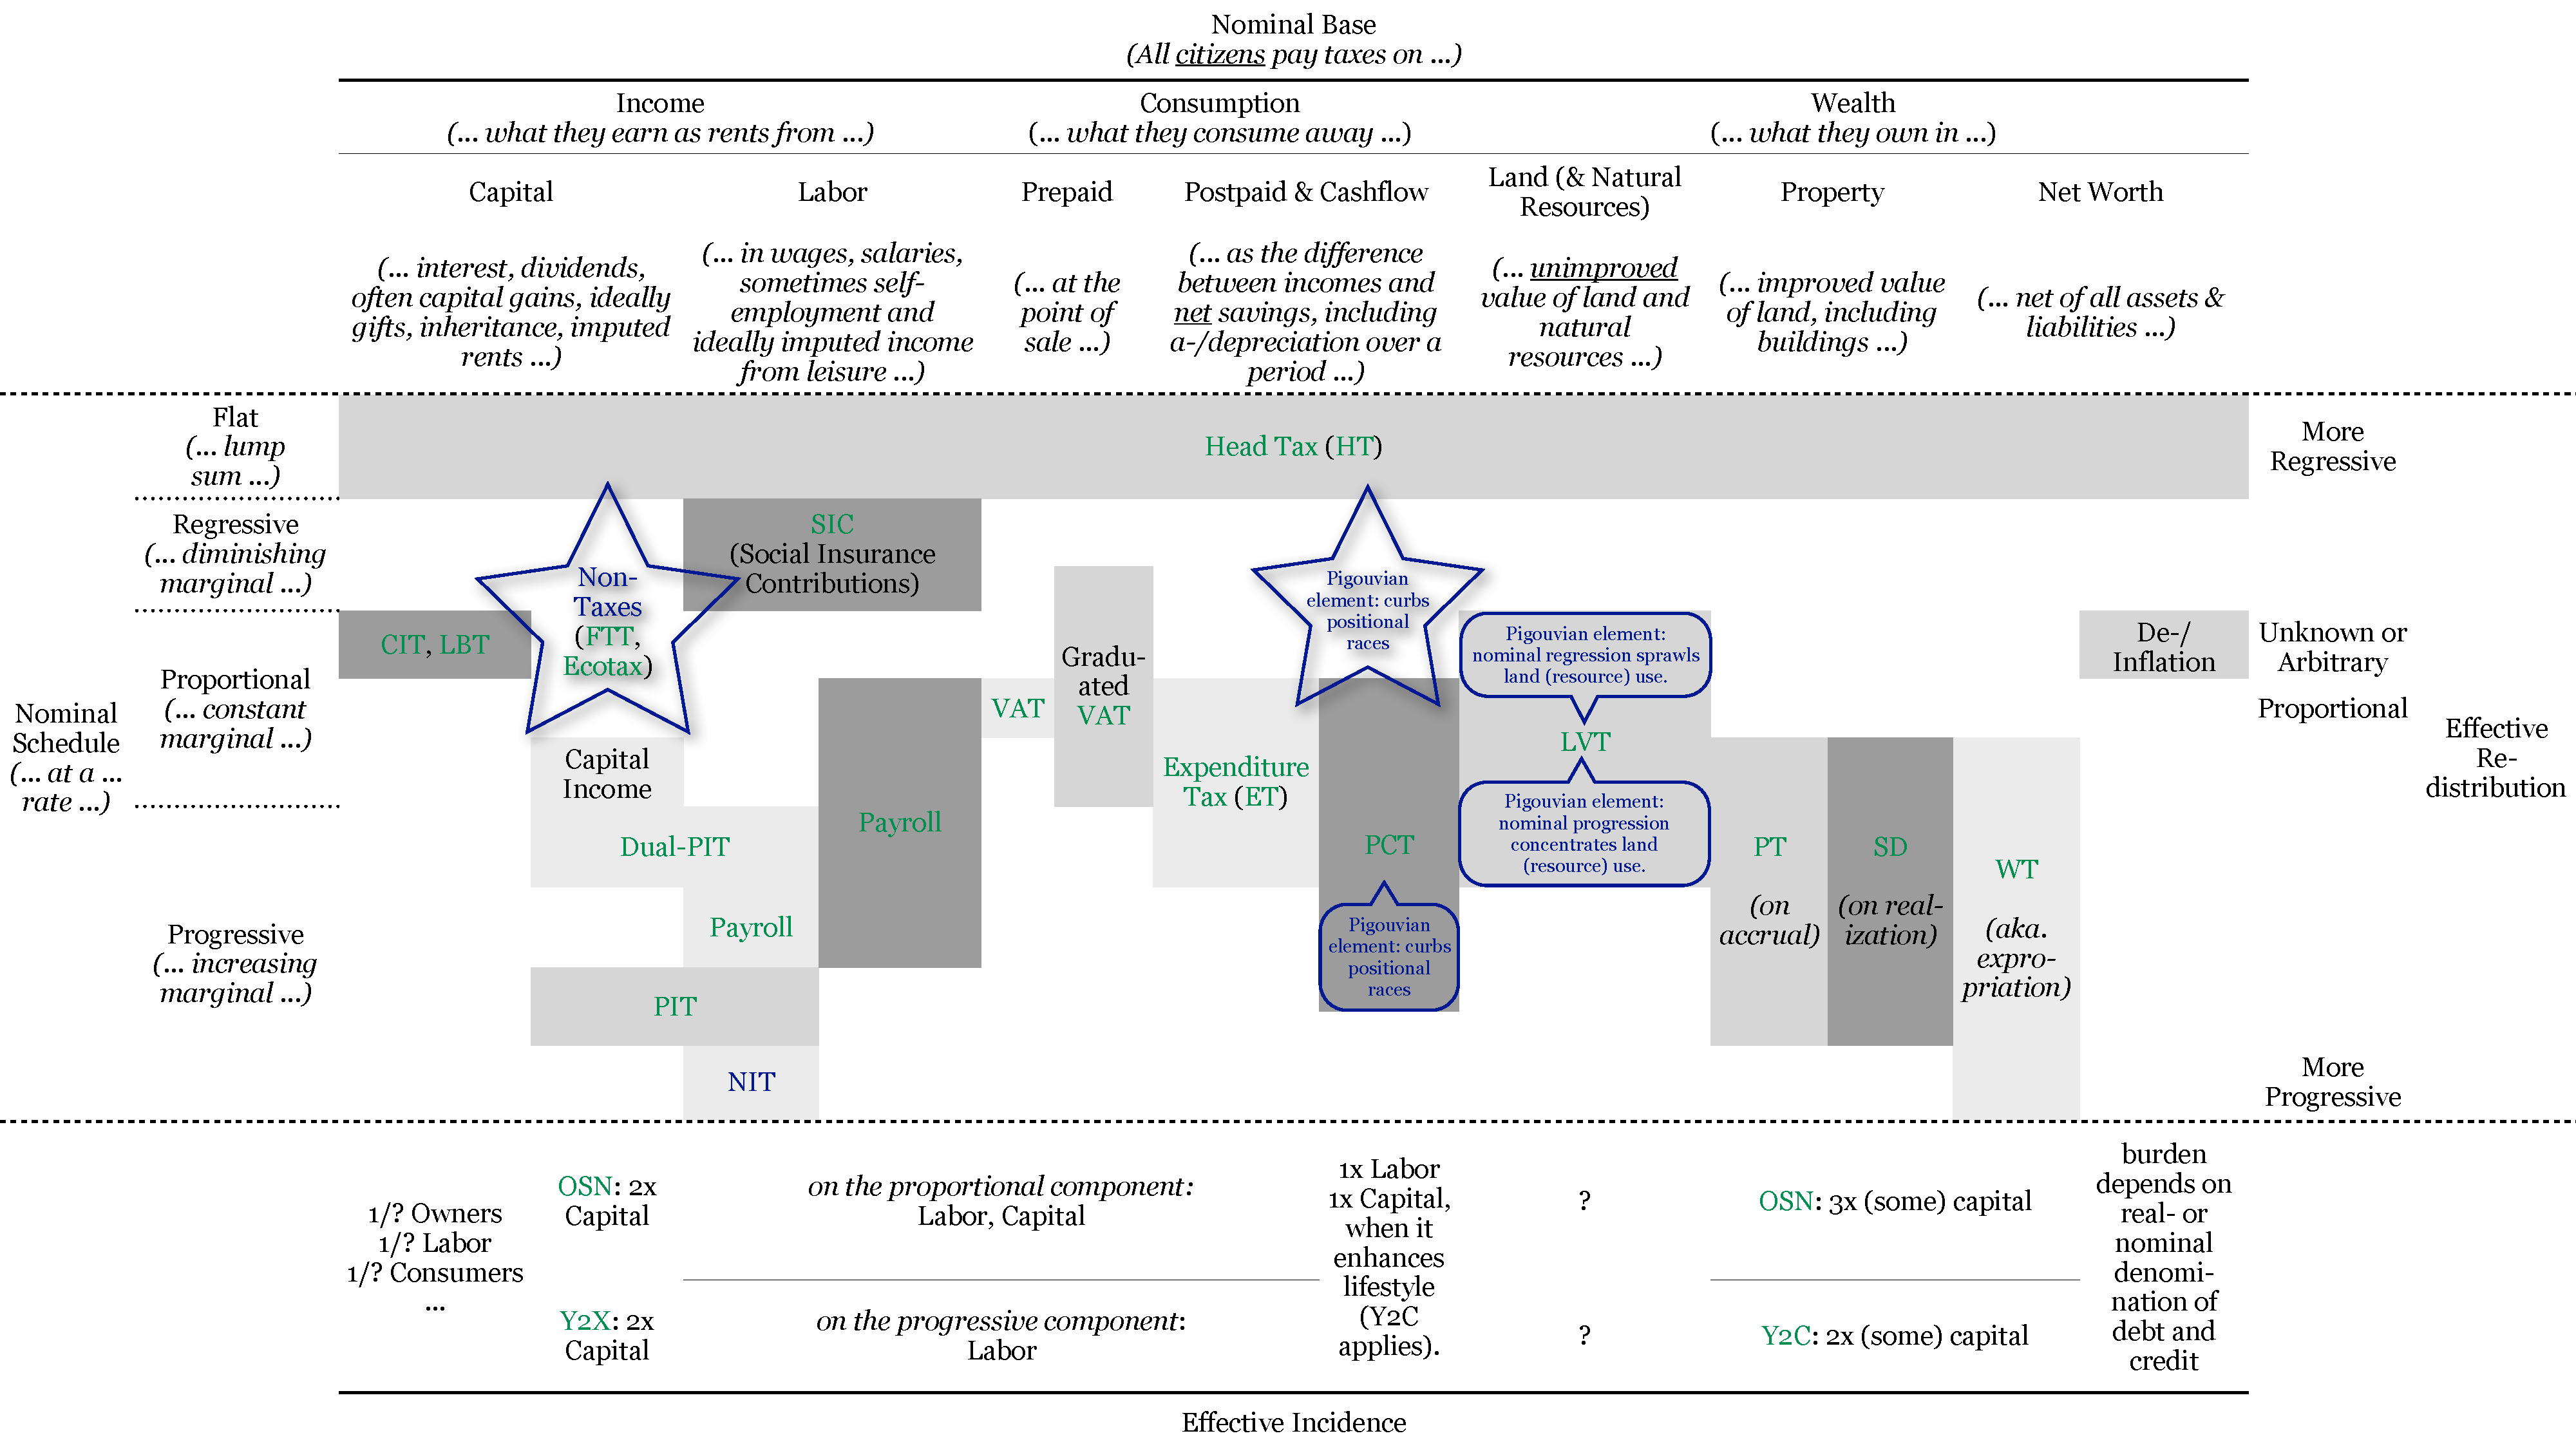
\includegraphics[width=1\linewidth]{tax-overview}  
	\caption{Incidence and Redistribution of Modern Taxes}
	\label{tab:tax-overview}
	\end{center}
	%!TEX root=../tax-democracy-held.tex

\scriptsize{
	\glsfirst{CIT},
	\glsfirst{Dual-PIT},
	\glsfirst{Ecotax},
	\glsfirst{ET},
	\glsfirst{FTT},
	\glsfirst{LBT},
	\glsfirst{LVT},
	\glsfirst{NIT},
	\glsfirst{OSN},
	\glsfirst{PCT},
	\glsfirst{Payroll},
	\glsfirst{PT},
	\glsfirst{SD},
	\glsfirst{VAT},
	\glsfirst{WT},
	\glsfirst{Y2C} and

	\hyperref[sec:distributive-effects-of-inflation]{the distributive effects of in- and deflation} (p.~\pageref{sec:distributive-effects-of-inflation}).
}
\end{figure}
\end{landscape}

If their democratic rule is to be enlightened, deliberators must also engage a set of abstractions concerning its optimality, justice and sustainability as well as problematize the view of human motivation, utility and rationality implied by these (economic) abstractions.
Deliberators must also understand the means and ends of an (ideal) mixed economy within which taxation reconciles allocation by plan and by exchange, including respective government and market failures.
Any deliberation that fails to engage these broadly consensual --- if not entirely coherent --- concerns, must be considered unenlightened. 
It would ignore some of the causal relationships and moral alternatives that we must assume exist, if and to the extent that we accept the economic ontology of coexisting states and markets.

\paragraph{Deliberation}
Deliberation is no such catalogue of first-order considerations of what would make a good (efficient, fair, sustainable) decision in any given policy field, but instead, a second-order prescription to resolve disagreement \emph{over} those very the moral and causal arguments \citep[125]{GutmannThompson-2004-aa}.
Still, and in contrast to pluralism, it places more than just \emph{procedural} claims, but posits \emph{substantive} requirements for how agreement must be reached.
Succinctly, \citeauthor{GutmannThompson-2004-aa} demand that ``your fellow citizens must give reasons that are comprehensible to you'' \citeyearpar[K177]{GutmannThompson-2004-aa}.
More than merely intelligible, permissible arguments to reach deliberative agreement must raise validity \citep{Habermas-1984-aa} and moral \citep{Rawls-1971-aa} claims \emph{universally} acceptable to everyone.

Logically, it must then be theoretically possible for any \emph{given} argument to fail that test, and to be impermissible --- including the arguments brought forward by experts.
In fact, deliberation reserves no special place for nominal experts at all, except if and to the extent that these experts have arrived at, and present their agreement under the standards of deliberation\footnote{
	As this PhD student can attest, there can be some doubt about whether (German social) science is really ruled by nothing but the ``unforced force of the better argument'' \citep{Habermas1984}.}.
	
As noted in the above, any research design that axiomatizes any disagreement between experts (or ex-ante logic) as \emph{misunderstandings} on the part of the non-experts fails the deliberative standard, no matter the supposedly enlightening de-biasing treatments.

\paragraph{Reciprocity}
The desiderata of taxation and deliberation are seemingly in conflict.
Taxation requires people to consider an exogenously given catalogue of abstractions, and deliberation implies that no such set of arguments can be unconditionally accepted.

This impasse has real repercussions for the proposed research design: apparently, it can serve only one master.
Either, participants misunderstandings can be revealed by treating them with introductory economics, \emph{or} they can deliberate any which arguments they themselves find comprehensible.

%\citep[4]{GutmannThompson-2004-aa}: ``A deliberative justification does not even get started if those to whom it is addressed cannot understand its essential content. It would not be acceptable, for example, to appeal only to the authority of revelation, whether divine or secular in nature.''

As with so much that deliberative theory is up against
\footnote{
	For example, political participation versus enlightened understanding versus political equality, as \citeauthor{Fishkin2009} points out.
}, %correct this
this is a false dichotomy.

Argumentative reciprocity implies that expert knowledge be neither presumed, nor negated, but that these arguments --- as all others --- be allowed to demonstrate their universal causal and moral validity.
Expert- and non-expert (as all other) arguments must not merely be balanced in terms of airtime or affect, but ``the considerations offered in favor of, or against, a proposal, candidate or policy [must] be answered in substantive way by \emph{those who advocate a different position}'' \citep[K550, emphasis added]{Fishkin2009}.
Deliberation is, in other words, when non-experts answer expert arguments \emph{on their own, expert terms}, and vice versa, too.
Surely, the relation of this ideal to practice is ``aspirational'', too, as all in deliberation \citep[K2679]{Fishkin2009} 
\footnote{
 And maybe, in democracy, too, as William H. Hastie (1904-1076), the first African American Justice on the U.S. Supreme Court warned us:
 \begin{quote}
 	\emph{``Democracy is not being, it is becoming. It is easily lost, but never finally won''.}
 \end{quote}
}.
Still, for the deliberative experimenter, this aspiration is the ultimate hypothesis in need of falsification.
If expert knowledge on taxation is presumed valid, and any dissent chalked up as misunderstandings the aspiration of communicative action could \emph{never} be falsified.
Likewise, if expert knowledge on taxation is not given adequate opportunity to be reciprocally considered on its own terms, communicative action will \emph{always} be violated.
Neither of those formats would provide construct-valid deliberation.

Instead, a deliberative format on taxation must enable participants to the farthest extent possible to argue expert as well as non-expert claims on their own terms, but must equally allow participants to ultimately reject either of those.

\subsection{Format}
Consequently, a good format for deliberating tax includes a strong learning component, where participants are introduced to the structured choices and relevant abstractions suggested by experts, including their disagreements, conditions and uncertainties.
Deliberators are unlikely to cover these extensive grounds by themselves, or pick them up from (very limited) briefing books and will benefit from well-planned lessons.
On the other hand, a good format must also feature extensive small-group discussion, where participants talk amongst themselves, shielded from the authority of expertise.
Deliberators may benefit from a trained, non-expert moderator and/or scribe to assist, structure and document their discussion.
Most importantly, participants must be encouraged to adjudicate the validity claims of economics, to contrast and possibly relate those to their own, and other claims.

As noted earlier, most deliberative formats include --- often moderated --- small-group discussion, but few add to that a substantive learning component\footnote{
	\glspl{DP}, the pronounced methodological gold standard of deliberation \citep{Mansbridge2010} are too short to feature long lessons, and confine expert knowledge to ad-hoc expert panels and limited briefing books \citep{Fishkin2009}.
	Citizen Juries \citep{SmithWales-2000-aa}, Planning Cells \citep{Dienel-1999-aa} and related formats also include no learning components, and some experimenters even advise against expert knowledge.}. %add source
Among those that do are the small-n Danish-developed Consensus Conferences \citep{Grundahl1995} and especially the large-n, one-off \gls{CA} in British Columbia, Canada \citep{Citizen-2004-aa}.
Consensus Conferences have been held on very technical issues, including nanotechnology \citep{LeeKleinman2007} or genetically modified foods, and the Citizen Assembly was tasked to recommend an alternative electoral system for the province.
Much like taxation, technology policy, and especially electoral systems design also demand highly structured choices  (for example, a seat allocation rule or regulation) and raises a set of abstractions (party systems or risk distributions).

In a Consensus Conference, 12-15 self-selected but diverse citizens discuss a technical matter of political relevance for three or more days (!) and issue a report on their discussions \citep{LeeKleinman2007}.
In preparation for the conference, participants read quite extensive background material, which they discuss during the first of several daylong sessions. 
At later sessions, they (publicly) share their questions with experts and finally draft a report for the sponsoring body and/or the media.
\citeauthor{LeeKleinman2007} report that a positive atmosphere, good organization and skillful facilitation are necessary for a successful Consensus Conference.
They also recommend that participants tell their stories, which moderators then weave into themes, to help citizens relate their experiences to expert knowledge \citeyearpar[159]{LeeKleinman2007}. 

The Citizen Assembly expanded on this model. 
Over the course of a year, 160 randomly selected British Columbians read and learned about electoral systems, held public hearings, deliberated amongst themselves and, after several intermediate votes, recommended a (quite complicated) \gls{STV}-variant and drafted a report \citep{Citizen-2004-aa}.
The extensive learning phase, spanning six (!) weekends stands out among deliberative experiments.
In addition to a university-level textbook on electoral systems, Citizens received interactive lectures accompanied by small discussion groups. 
An expert panel vetted the learning phase for impartiality and accuracy of information.
Participants also developed a set of shared values during the learning phase, both (procedurally) for how they wished to deliberate and (substantively) for a desirable electoral system.

\subsection{Implementation} 

The \gls{CA} provides an ideal blueprint for a deliberative forum on tax; however, limited resources and lack of experience do not permit such a large undertaking for this project.

Instead, the project proposed here is a scaled-down hybrid, combining the ambitious learning phases of a Citizen Assembly
\footnote{
	The \gls{CA} also featured a ``listening phase'' \citep[1609]{Pearse2008} during which members held public hearings throughout the province, drawing some 3,000 attendees and 1,600 written submissions. 
	Both because I do not have the resources and --- absent a mandate --- expect limited public interest, I plan no such phase.
}
, with the more intimate, small-n interaction and participant empowerment of Consensus Conferences.

A small, self-selected sample of 8-12 diverse citizens will attend 5-8 days of learning and deliberation spread over several weeks. 
%\cite[K2485]{Pearse2008} speak of an ``epistemological deficiency, by failing to incorporate insights supplied by different group perspectives.''
During the learning sessions, taking up less than half of the time, participants receive information about the structured choices and relevant abstractions of taxation from the author.
These lessons are organized around themes and values identified by deliberators in an initial session, and attempt to relate the subject matter to participant experiences.
Learning sessions alternate with extensive small-group deliberations, during which participants reflect on the lessons, relate or contrast it to their own experiences and claims and adjudicate the validity of the presented moral and causal arguments.
Small-group deliberations are facilitated by a trained moderator, who has no expertise in taxation or economics.
At the end of the process, participants must vote on a tax regime and write a report of their deliberations.
If resources permit, participants will also hear a panel of expert witnesses to discuss their questions.

The forum will be run twice, for two extreme case samples: once as an undergraduate class at the University of Bremen, and once as an adult evening class with the Volkshochschule and/or in association with organized labor.
Participants in the university class will be graded, but not based on their contributions to the deliberations, to which the author and instructor will not be a party. 
The class will be advertised through the usual channels at the university.
Participation in the adult evening class will be free of charge, deliberators may be reimbursed for local travel, receive free food and will be offered childcare. 
The class will be advertised through local organized labor to attract non-academic participants.




%a good format for my goal includes 
    %Includes a strong learning component, structured roughly along my drafts -- but shorter, and in more accessible style. (It must not be a microeconomics text).
    %Relates these abstractions to personal experiences and intersubjective value judgments.
    %Prioritizes intensity (duration) over representativeness (sample size) under given constraints (time, money).
    %May involve me and existing material for the learning component, but someone else must moderate the deliberations.
    %Starts from a small-scale, face-to-face deliberation as a pilot study, both to guarantee concept validity and because I have no idea about deliberation-

    %Instead the same quasi-experimental design could be run with qualitative data, including, open-ended questionnaires and/or semi-structured interviews, or even a record of the deliberations. Such data could be content-analysed (or rather: coded) to distill the (mis)understanding before and after the treatment.


%note rosenberg on "by no means unimportant"
%note reciprocity, sharing ones causal assumptions

%note that the link between rosenbergs sequence thinking and my tax misunderstandings is still to be developed

%\cite{Johnson1998}
    %161: ``Would-be political reformers of various persuasions urge deliberation upon us. Yet in their pleadings such theorists and reformers frequently invoke deliberation in an uncritical manner. They proceed as though the ways in which deliberation and the effects we can expect of it are not just obvious, but attractively so.''
	
%\cite{Azmanova2010} (also \cite{Fishkin2009}: 529)
	%49: thoughtfulness and reflexivity (as per Fishkin) require 1) reasonably accurate information 2) substantive balance 3) diversity, 4) conscientiousness, 5) equal consideration

%\cite{Citizen-2004-aa}
	%11: one guy did the learning sessions
	%1) has a selection phase
	%2)  has a LEARNING phase
		%also develop "shared values" about the process
	%3) has a PUBLIC HEARING phase
	%4) has a DELIBERATION phase
	%go to chrch with group, maybe.

	
%\cite{Fung-2003-ac}
	%very good summary, get back to this
	
%\cite{Fishkin2009}
	%democracies are supposed to fulfill two values; political equality and deliberation (loc. 84)
	%``a democracy in which we all had substantive information [and] [\ldots] substantive opinions would seem to take too many meetings.''
	%what's wrong with unenlightened opinions (all loc. 113ff)
		%\begin{enumerate}
			%\item they may be volatile (cite other sources
			%\item people may be manipulated by foregrounding some information (clean coal vs. dirty coal, forgetting about natural gas -- compare this to tax choice)
			%\item misinformation (savings rate)
			%\item favor favorable, true arguments over others
			%\item manipulation may ``prime'' one aspect of policy.
		%\end{enumerate}
	%loc 260: ``the hard choice, in other words, is between debilitated but actual opinion, on the one hand, and deliberative but counterfactual opinion, on the other.''
	%loc 369: table with raw/refined opinion, and different kinds of sampling.
	%loc 438: ``The idea is that if a counterfactual situation is morally relevant, why not do a serious social science experiment -- rather than merely engage in informal inference or armchair empiricism -- to determine what the appropriate counterfactual situation might look like? and if that counterfactual is both discoverable and normatively relevent, why not then let the rest of the world know about it? Just as John Rawls's original position can be thought of having a kind of recommending force, the counterfactual representation of public opinion identified by the \gls{DP} also recommends to the rest of the population some conclusions that they ought to take seriously.''
	%loc 390: self-selected samples will be very limited in what they can achieve.
	%loc 401: citizen juries use quota samples, consesus conferences use self-selected samples, then with some quota sampling
	%loc 550: notes that positions must not merely be balanced in terms of airtime or affect, but ``whether the considerations offered in favor of, or against, a proposal, candidate or policy are answered in a substantive way by those who advocate a different position.'' %THIS IS KEY!
	%loc 561: three categories for such considerations
		%``the benefits or burdens of a policy or political choice,
		% the causal arguments about whether those benefits or benefits or burdens will actually result from one choice or another,
		%and the values by which those benefits and burdens might best be evaluated.''
		%loc 1424: ``the problem is that any microcosmis deliberation taking place in a modern society will be one in which there are significant social and economic inequalities in the conduct of ordinary life in the broader society.
		 	%It seems difficult or impossible to `bracket' these inequalities -- for participants to behave `as if' they do not exist. 
		 	%Indeed the problem goes deeper. The possibility of doing so is the challenge of the ``autonomy of the political'', namely, whether or not equality can hold sway in politics in a world in which inequality rules in economic and social relations.
		 	%The viability and legitimacy of the liberal-democratic process may turn on the answer.'' \citep[loc. 2679]{Fishkin2009}

%\cite{GutmannThompson-2004-aa}
	%loc177: `your fellow citizens must give reasons that are comprehensible to you''
	%loc 188: they introduce first and second-order theories, too!
	%loc 919, writing about Fish: ``Giving reasons is the chief way of academics to exercise power in democratic politics. All the talk about deliberation, like deliberation itself, is merely a cover for power politics.''.
		
%iris marion young, especially notes that people of lower status may have a hard time getting listened to, or that others may be particularly accustomed to orderly forms of reason-giving arguments that weigh with other participants -- and this may be particulary problematic the more substantive the topic is.

%note that 

%groupthink!

%tax allows only very limited choice: income, consumption or assets; a couple of schedules, plus some pigouvian taxation.  the CIT, notably, is just a special way to raise the PIT. Otherwise, only natural persons. Tax demands these choices. Also, these choices \emph{are} as I explain in the below, political, so they must be made legitimately, and we may not be able to simply outsource them to elites.

%Note how the DP on energy -- which, at first, seems similar -- is actually not. It asked, among other things, whether people would be willing to pay more on their monthly utility bills for wind \citep[loc. 2013]{Fishkin2009}, but not more technical stuff than that.
	
%argue exactly why small sub-issues of tax do not work; they violate the real choices.

%there remain problems: you can't just go about this as if it wwere not controversial; it is controversially maongst experts, but more importantly, controversial whether experts have in fact authority and the right context. It can't just be an experiment, or a treatment intervention where ordinary citizens must necessarily become more like experts, and if they are not, then the teaching has failed. It must be possible for people to disagree with the abstractions they ar epresented with, see the criticism of it.

%tax is very technocratic, simply because the instition is like that.
%this will have to be qualitative

%\gls{OECD}-world (\autoref{chap:3-crises}

%Tax offers/demands very structured choices: there are essentially only 4x3 broad tax types (see tax table in drafts). Different from, for example, a deliberation on “racial tensions”, deliberating tax choice is more close-ended.
%Tax expertise is easily politicized, because:
%Tax cannot be reduced to an empirical question, both because inframarginal data is not available, and because macroeconomics is incompletely understood.
%Tax cannot be reduced to a consequentialist inquiry, because people (may) care about other normative claims, too (e.g. fairness). 

%Tax cannot be easily (if at all) dumbed down to subsets of tax choice (e.g. VAT vs PIT), or subsets of abstractions (e.g. only “bastard keynesianism”) for two reasons:
    %Any such reduction would violate the spirit of deliberation; citizens could not set their own agenda.
    %Any such reduction may well fail to elucidate my hypothesized misunderstandings: I imagine “understanding tax” as a bucket, which, if leaky will drain to the lowest level. For example, if deliberators would discuss most aspects of taxation, but skip over the limits (!) of price controls, they may well opt for price controls in lieu of, or in addition to taxation


\section{Research Design}
%see below
%cases, people, selection
%methods of observation and/or inference

\subsection{Hypotheses}
The threefold research question raises several hypotheses:

%Both research questions \ref{itm:resolve-better-tax} and \ref{itm:prove-deliberative-democracy} can be rolled up in one set of hypotheses:

\begin{enumerate}
    \item \label{itm:think-different}
		If ordinary citizens are given the possibility to deliberate welfare and taxation, they will think differently about it.
		Specifically,
		\begin{enumerate}
		
			\item \label{itm:knowledge-gain}
				\emph{Knowledge Gain.}
				People will gain in knowledge.
				Specifically relevant for tax choice (\autoref{fig:tax-with-misunderstandings}, p.~\pageref{fig:tax-with-misunderstandings}),
				\begin{enumerate}
				
					\item \label{itm:bastard-keynesianism} 
						\emph{Bastard Keynesianism.}
						People will understand that an economy can have an arbitrary (sub-\citeauthor{Solow1956}) savings rate, and that --- equivalently --- if lowered slowly, aggregate \emph{consumption} will not depress aggregate \emph{demand}.
				
					\item \label{itm:real-myopia}
						\emph{Real Myopia.} %aka technocratic myopia
						People will understand that the future prosperity of an economy is, in part, determined by present \emph{net} investment, and that --- equivalently --- \emph{real}, not \emph{nominal} (for example, \gls{GDP}) indicators track the savings rate of an economy.
				
					\item \label{itm:bastard-hayekianism} %aka government vs markets
						\emph{Bastard Hayekianism.} %make naming consistent
						People will understand that an economy can adopt an arbitrary government quota (if, possibly, at a cost), and that --- equivalently --- not \emph{all} (but some) taxed resources are lost.
						Taxation is not exclusively or unconditionally a negative-sum proposition.
				
					\item \label{itm:flyper-theory} %aka tax-aversion
						\emph{Flypaper Theory.}
						People will understand that ontologically and empirically, only and always \emph{natural} persons bear the burdens of taxation, and that --- equivalently --- the flypaper theory of tax incidence is false.
						
						This hypothesis is similar to, but not identical to \citeauthor{McCafferyBaron2003}'s findings of \emph{tax aversion}, by which people mistakenly prefer taxes not labeled as such and/or indirect taxes and a \emph{disaggregation effect}, by which people fail to integrate taxes on same bases.
						%might have to feature tax aversion separately, because that is already in the visualizatiuon
				
					\item \label{itm:ordoliberal-mess}
						\emph{Ordoliberal Mess.} %not hygiene, that's the opposite
						People will understand that Pigouvian and general-revenue taxes follow opposing logics, and that --- equivalently --- a Pigouvian tax \emph{should not} raise revenue.
						
						This hypothesis is similar to, but not identical to \citeauthor{McCafferyBaron2003}'s findings of a \emph{disaggregation effect}, by which people fail to integrate different taxes even on same bases.  %this is (\cite{McCaffery2003}: 19ff)
						%is this really right?
						
					\item \label{itm:false-omnipotence}%clarify labeling
						\emph{False Omnipotence.} %used to be negative some 
						People will understand that taxation will often (if not always) cause unintended consequences in markets, or that --- equivalently --- taxation can cause a negative-sum \gls{DWL}. 
						Taxation is not exclusively or unconditionally a zero-sum proposition.
						
					\item \label{itm:false-omniscience}
						\emph{False Omniscience.}
						Relatedly, people will understand that taxable income and wealth (but not consumption) cannot be measured independent of market-pricing, or that --- equivalently --- any taxation based on fiat evaluations may have unintended consequences in markets.
				\end{enumerate}
			
			\item \label{itm:universal-validity}
				\emph{Universal Validity}
				People will find the above abstractions meaningful and accept a universal validity of underlying causal and moral arguments.
			
%			\item \label{itm:preference-structuration}
%				\emph{Preference structuration.}
%				Partly as a function of the above knowledge gain, people will have better-structured preferences over taxation.
				
%				Specifically, and related to the cyclical preferences \citep[334]{Farrar2010} and other aggregation failures of pluralist democracy \citep[for example,][]{Condorcet1785,Arrow1963},

%				\begin{enumerate}
					
%					\item \label{itm:vNM-consistent}
%						\emph{\glsfirst{vNM}-Consistency.}
%						\emph{Individually}, people will have ordinal preferences that more closely resemble \gls{vNM}-consistency.
				
%					\item \label{itm:single-peakedness}
%						\emph{Single Peakedness.}
%						\emph{In the aggregate}, people will have preferences that more closely resemble single-peakedness.
				
%					\item \label{itm:orthogonal-dimensions}
%						\emph{Orthogonal Dimensions.}
%						\emph{In the aggregate}, people will have preferences that more closely resemble orthogonal factors.
%				\end{enumerate}
				
			\item \label{itm:attitude-change}
				\emph{Attitude Change.}
				Partly as a function of the above effects (as in \autoref{fig:tax-with-misunderstandings}, p.~\pageref{fig:tax-with-misunderstandings}), people will prefer a \glsfirst{PCT}, conditionally supplemented by a \glsfirst{WT}, \glsfirst{LVT} and \glsfirst{NIT} over the present tax regimes of \glsfirst{PIT}, \glsfirst{VAT} and \glsfirst{Payroll}.
		\end{enumerate}
	
	\item \label{itm:interaction-effects}
		\emph{Interaction Effects.}
		The above effects will:
			\begin{enumerate}
				\item \label{itm:interact-equity}
					\emph{Not interact} with people's equity beliefs, or --- equivalently --- people will not change their thinking about tax as a function of their allocative preferences.
				\item \label{itm:interact-ses}
					\emph{Interact negatively} with people's socio-economic status, or --- equivalently --- people with greater socio-economic status will change their thinking about tax the least.
				\item \label{itm:interact-cognitive-ability}
					\emph{Interact negatively} with people's cognitive ability, or --- equivalently --- people with less cognitive ability will change their thinking about tax the least.
			\end{enumerate}
\end{enumerate}
    
%\begin{landscape}
% \begin{figure}[htbp]
%    \begin{center}
%	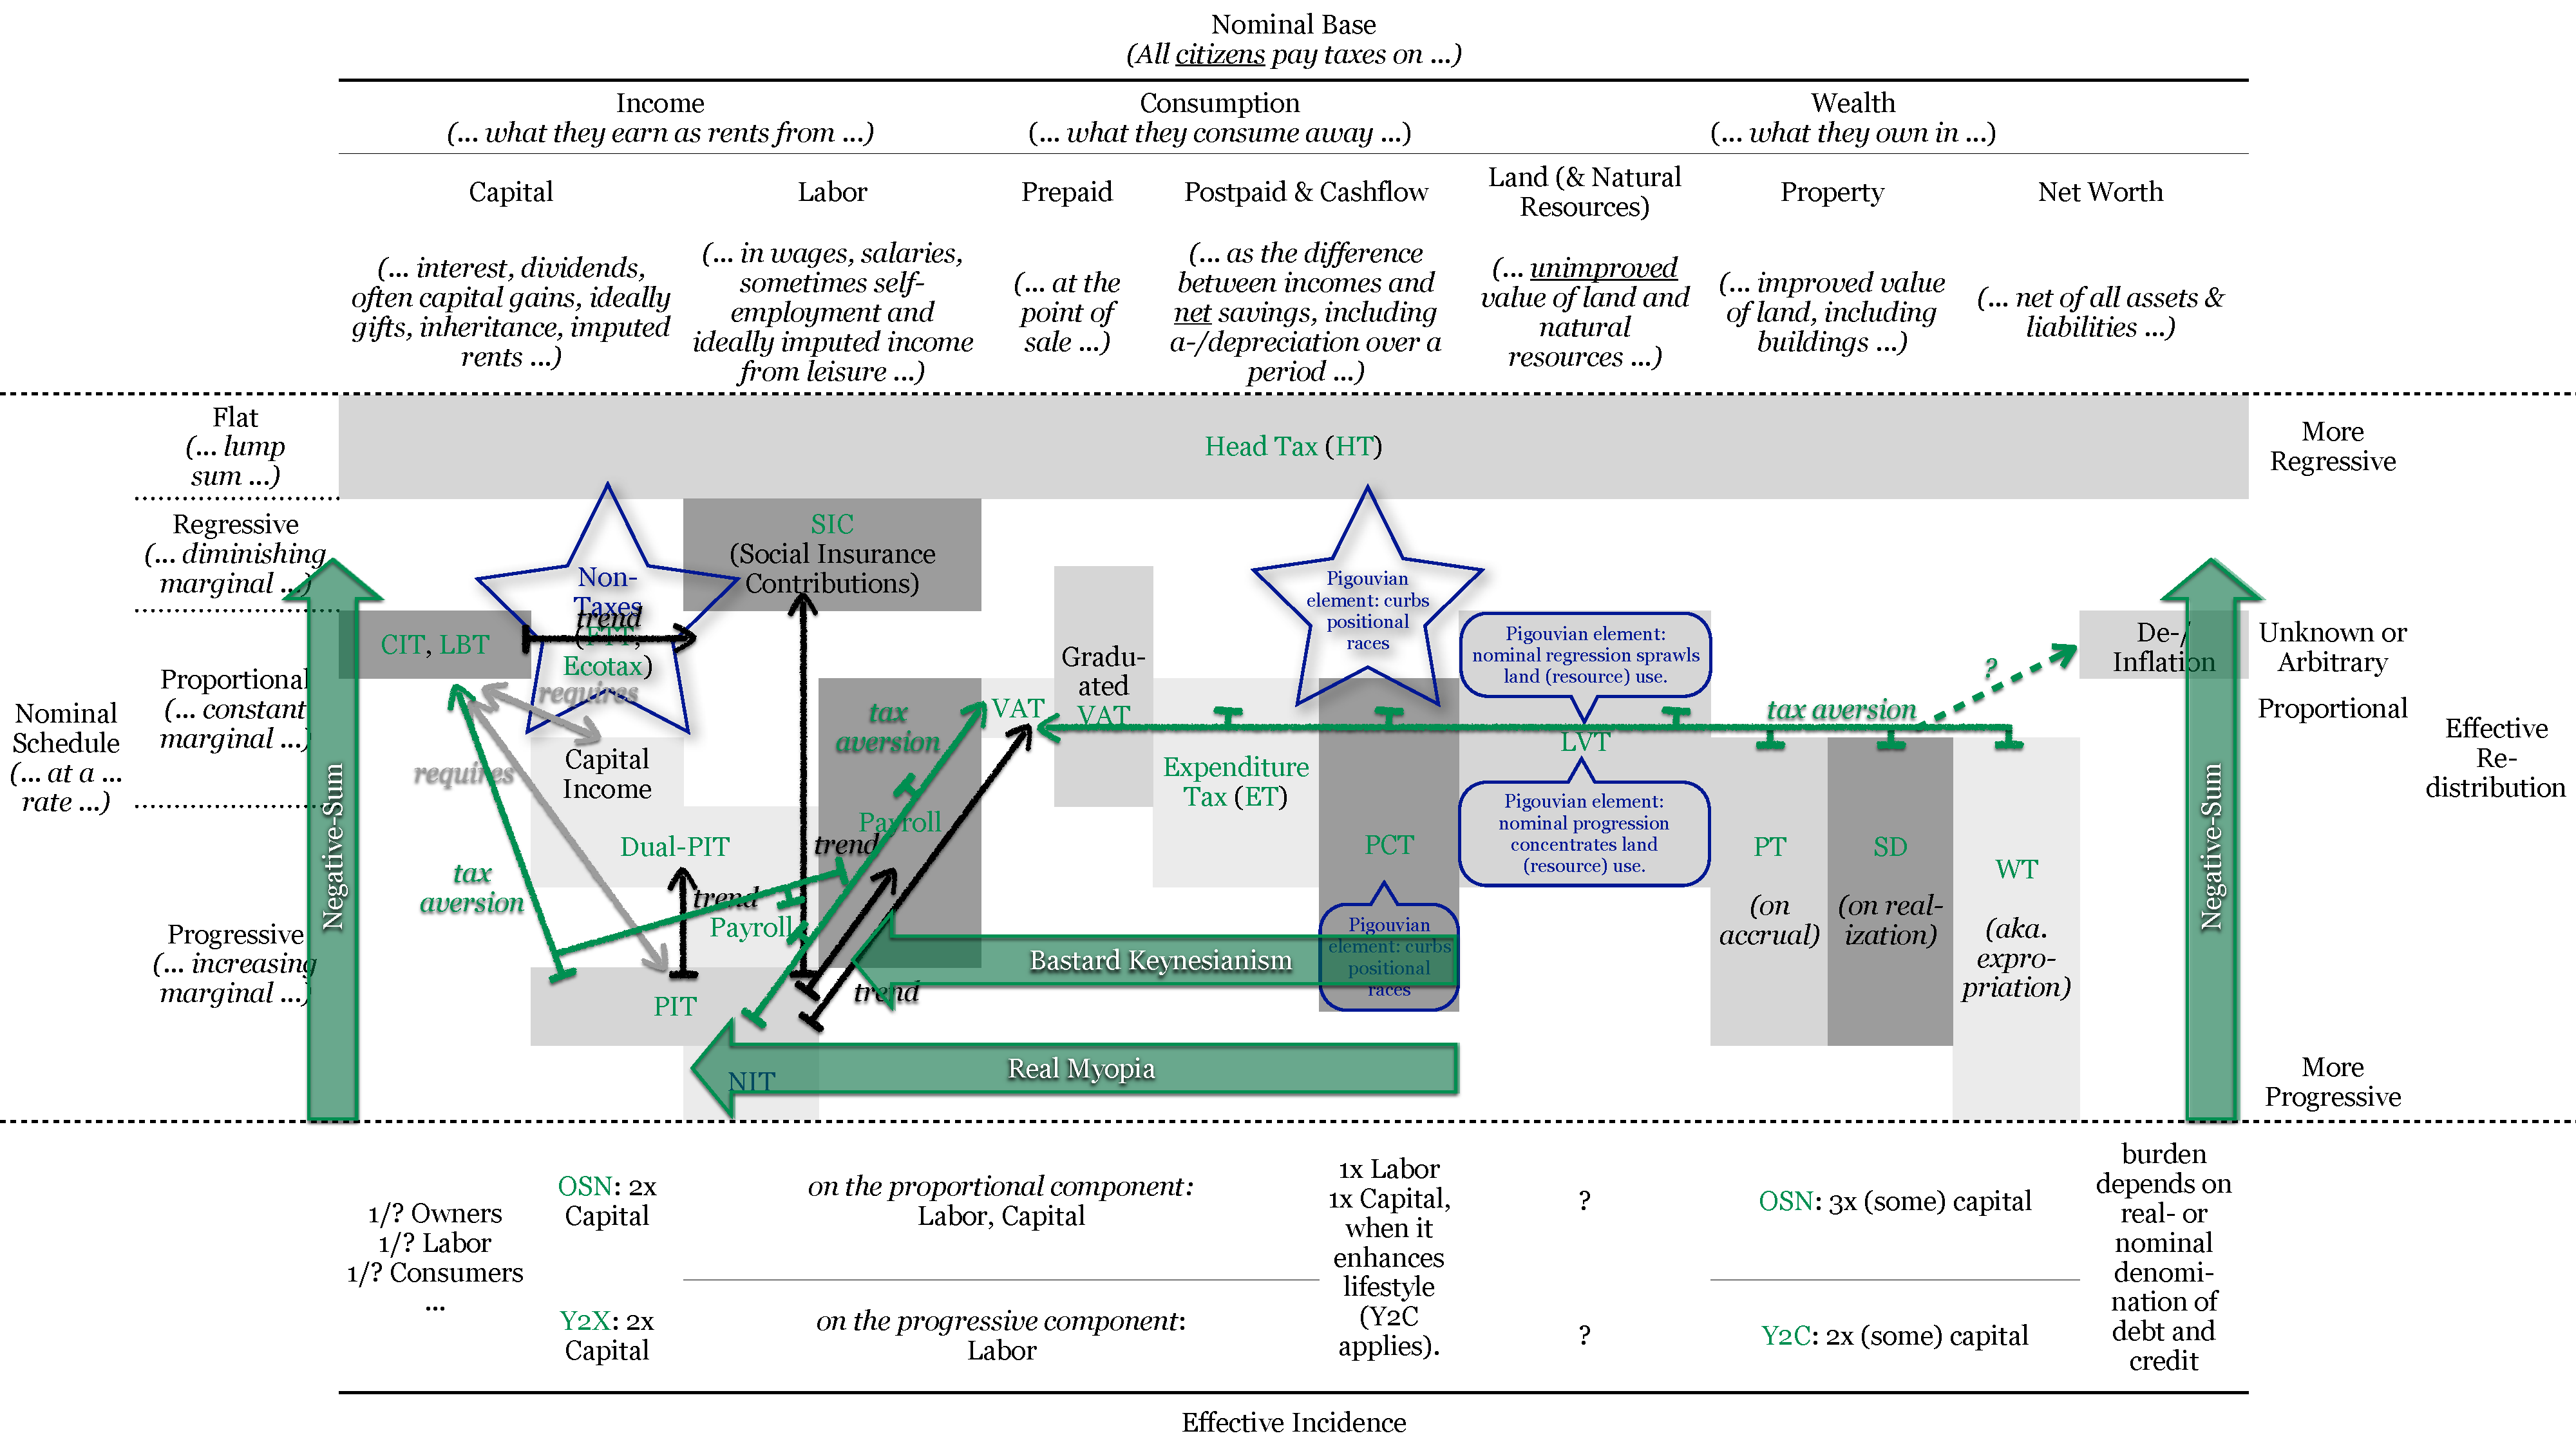
\includegraphics[width=1\linewidth]{tax-with-misunderstandings}  
%	\caption[The Vector Field of Taxes with Misunderstandings]{The Vector Field of Taxes with Misunderstandings}
%	\label{fig:tax-with-misunderstandings}
%	\end{center}
%%	%!TEX root=../tax-democracy-held.tex

\scriptsize{
	\glsfirst{CIT},
	\glsfirst{Dual-PIT},
	\glsfirst{Ecotax},
	\glsfirst{ET},
	\glsfirst{FTT},
	\glsfirst{LBT},
	\glsfirst{LVT},
	\glsfirst{NIT},
	\glsfirst{OSN},
	\glsfirst{PCT},
	\glsfirst{Payroll},
	\glsfirst{PT},
	\glsfirst{SD},
	\glsfirst{VAT},
	\glsfirst{WT},
	\glsfirst{Y2C} and

	\hyperref[sec:distributive-effects-of-inflation]{the distributive effects of in- and deflation} (p.~\pageref{sec:distributive-effects-of-inflation}).
}
%\end{figure}
%\end{landscape}

\subsection{Data and Methods}
To clearly measure the hypothesized $\Delta$ in knowledge and preferences, but also to verify argumentative reciprocity and to directly observe (or problematize) communicative action, this project will utilize both survey and process data.

Akin to the \gls{DP}s, participants will be asked to respond to closed- and open-ended survey questions on tax issues, both before and after the forum.
The surveys will also gather basic socio-economic data and invite feedback on the deliberative forum itself.
This data can be compared before and after the deliberative treatment within-subjects.
Lacking a sufficiently large sample, in lieu of quantitative analysis of closed-ended questions, responses to open-ended questions will be qualitatively coded and compared with the hypothesized (mis)understandings.

Additionally, process data from the deliberation will be gathered, comprising of the claims, themes and questions raised by participants and summarized by the moderator and/or scribe at the end of each deliberation, as well as the final report on taxation and other documents or notes produced during the deliberation.
Deliberations will also be audio-(visually) recorded, although comprehensive transcription and analysis of this data will probably not be possible.
This process data and select recordings will then be subjected to a qualitative content analysis, both to verify that participants \emph{could} make arguments reciprocally comprehensible, and to record which of several arguments deliberators accepted as based on universal validity claims.

\section{Feasibility}
This project is theoretically, methodologically and organizationally demanding, but it can be completed in about 2 years.
In my prior work on the mixed economy and taxation, I have already distilled a compact set of abstractions and choices to be considered by deliberators.
Existing chapters (4-8) provides a good basis for the briefing material, learning phases, questionnaire development and qualitative analyses.
Happily, these chapters abstract away much of the political controversy over economic issues, clearly state remaining expert dissent and, rather than definitive answers, present a catalogue of questions, tradeoffs and clarifications.
Prior work and derived material should hopefully be roughly consensual amongst experts, and thoroughly balanced.
Still, additional vetting and advice from a panel of academic economists will be required, especially because my highly selective training is mostly auto-didactic.

While I have some experience teaching introductory classes on political economy, ensuring the deliberative autonomy of participants will be a challenge.
The two fora, even though organized as classes, must not regress to a (traditional) classroom setting in which the economics teacher knows best.
Because I have no practical experience with deliberative formats, ensuring conditions for genuine communicative action will be hard.
Together with the moderator and/or scribe, the two fora must be meticulously planned and discussed with experienced organizers.
Ideally, I should attend a deliberative experiment to gain some first-hand impressions.

Moreover, participant acquisition and sample attrition for the labor group will likely pose problems, requiring early planning and concerted outreach to local organizations and leaders.

Lastly, data gathering and analysis may easily outmatch available resources.
I must filter data and focus the analysis on a manageable size.

\section{Payoff}
This is probably an unconventional, and possibly risky project, but it has promise, too.

If, given the right design, deliberative democracy can enable citizens to rule on complex issues, by resolving their disagreements through communicative action, political scientists will have a very able, and attractive hypothetical to compare with, and deliberative experimenters should have more courage to venture out to more topics facing our sovereigns.
Not just as social scientists, but as citizens too, we must know whether the once historical achievement of aggregative democracy is now withering away under the assault of tightly concentrated special interest and obscuring complexity.
If it can show its stripes, deliberative democracy may well be our last, and also our best hope, to reveal the perils of pluralism, then to live up to our greater capacity for communicative action.

If, even under the brand of liberal democracy most demanding of political autonomy, people of lower cognitive ability or socio-economic status were to misunderstand taxation, be unable to engage in reciprocally comprehensible argument and as a result, opt for taxes against their material interest, social inequality research would face a whole new process of perpetuating privilege.
Not only as social scientists, but as citizens, too, we must know how no one gets left behind in our schools of democracy \citep{DeTocqueville1840,Rosenberg-2002-aa}.
Liberal democracy, at bottom, requires that political participation \emph{can} be made autonomous from power, status and wealth, and on this condition hinges the feasibility of liberalism as a political philosophy.

If, under a normatively more attractive democratic process, people were to resolve some misunderstandings about, and agree on different, but doable and desirable taxes, welfare state research and political economy would have to explain a much greater retrenchment and democratic failure.
Not only as social scientists, but as citizens, too, we must know that better tax we could agree on, and if it exists, what is keeping us from it.
Taxation, underneath it all, \emph{is} the social contract \citep{SchumpeterSwedberg-1942-aa}, and its vitality will determine the prospects for modern progress.

How, ask wryly \cite[2]{PrzeworskiSalomon1995}, will we ever know that such grandiose conclusions are valid?

Here, the project turns full circle, and back to reciprocity.
We will know that these conclusions are valid, if at every point along the way --- theory, operationalization, sampling, measurement and analysis --- I have provided causal and moral arguments that are universally acceptable.

I have provided reasons in this proposal; I hope they are comprehensible to my readers --- and especially to my supervisors.
Now, we must adjudicate their universal validity on their own terms.
With any luck, \gls{BIGSSS} will still be a place where such communicative action happens.